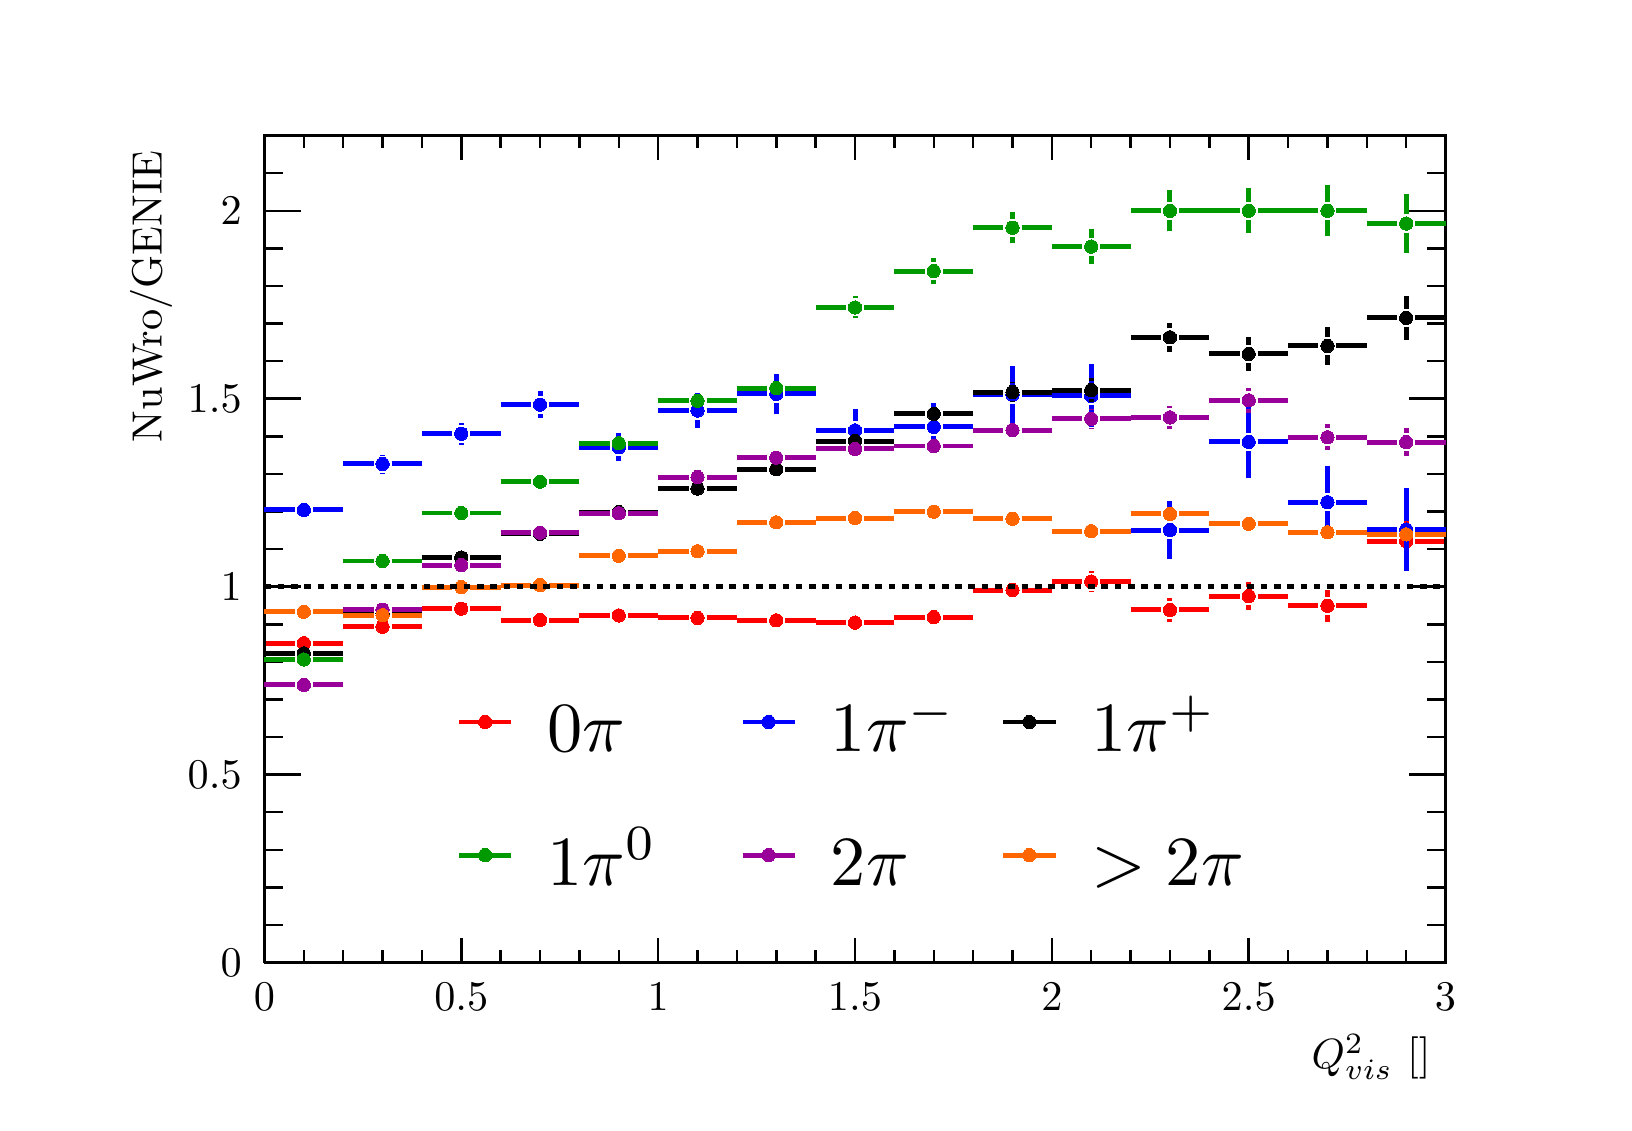
\begin{tikzpicture}
\pgfdeclareplotmark{cross} {
\pgfpathmoveto{\pgfpoint{-0.3\pgfplotmarksize}{\pgfplotmarksize}}
\pgfpathlineto{\pgfpoint{+0.3\pgfplotmarksize}{\pgfplotmarksize}}
\pgfpathlineto{\pgfpoint{+0.3\pgfplotmarksize}{0.3\pgfplotmarksize}}
\pgfpathlineto{\pgfpoint{+1\pgfplotmarksize}{0.3\pgfplotmarksize}}
\pgfpathlineto{\pgfpoint{+1\pgfplotmarksize}{-0.3\pgfplotmarksize}}
\pgfpathlineto{\pgfpoint{+0.3\pgfplotmarksize}{-0.3\pgfplotmarksize}}
\pgfpathlineto{\pgfpoint{+0.3\pgfplotmarksize}{-1.\pgfplotmarksize}}
\pgfpathlineto{\pgfpoint{-0.3\pgfplotmarksize}{-1.\pgfplotmarksize}}
\pgfpathlineto{\pgfpoint{-0.3\pgfplotmarksize}{-0.3\pgfplotmarksize}}
\pgfpathlineto{\pgfpoint{-1.\pgfplotmarksize}{-0.3\pgfplotmarksize}}
\pgfpathlineto{\pgfpoint{-1.\pgfplotmarksize}{0.3\pgfplotmarksize}}
\pgfpathlineto{\pgfpoint{-0.3\pgfplotmarksize}{0.3\pgfplotmarksize}}
\pgfpathclose
\pgfusepathqstroke
}
\pgfdeclareplotmark{cross*} {
\pgfpathmoveto{\pgfpoint{-0.3\pgfplotmarksize}{\pgfplotmarksize}}
\pgfpathlineto{\pgfpoint{+0.3\pgfplotmarksize}{\pgfplotmarksize}}
\pgfpathlineto{\pgfpoint{+0.3\pgfplotmarksize}{0.3\pgfplotmarksize}}
\pgfpathlineto{\pgfpoint{+1\pgfplotmarksize}{0.3\pgfplotmarksize}}
\pgfpathlineto{\pgfpoint{+1\pgfplotmarksize}{-0.3\pgfplotmarksize}}
\pgfpathlineto{\pgfpoint{+0.3\pgfplotmarksize}{-0.3\pgfplotmarksize}}
\pgfpathlineto{\pgfpoint{+0.3\pgfplotmarksize}{-1.\pgfplotmarksize}}
\pgfpathlineto{\pgfpoint{-0.3\pgfplotmarksize}{-1.\pgfplotmarksize}}
\pgfpathlineto{\pgfpoint{-0.3\pgfplotmarksize}{-0.3\pgfplotmarksize}}
\pgfpathlineto{\pgfpoint{-1.\pgfplotmarksize}{-0.3\pgfplotmarksize}}
\pgfpathlineto{\pgfpoint{-1.\pgfplotmarksize}{0.3\pgfplotmarksize}}
\pgfpathlineto{\pgfpoint{-0.3\pgfplotmarksize}{0.3\pgfplotmarksize}}
\pgfpathclose
\pgfusepathqfillstroke
}
\pgfdeclareplotmark{newstar} {
\pgfpathmoveto{\pgfqpoint{0pt}{\pgfplotmarksize}}
\pgfpathlineto{\pgfqpointpolar{44}{0.5\pgfplotmarksize}}
\pgfpathlineto{\pgfqpointpolar{18}{\pgfplotmarksize}}
\pgfpathlineto{\pgfqpointpolar{-20}{0.5\pgfplotmarksize}}
\pgfpathlineto{\pgfqpointpolar{-54}{\pgfplotmarksize}}
\pgfpathlineto{\pgfqpointpolar{-90}{0.5\pgfplotmarksize}}
\pgfpathlineto{\pgfqpointpolar{234}{\pgfplotmarksize}}
\pgfpathlineto{\pgfqpointpolar{198}{0.5\pgfplotmarksize}}
\pgfpathlineto{\pgfqpointpolar{162}{\pgfplotmarksize}}
\pgfpathlineto{\pgfqpointpolar{134}{0.5\pgfplotmarksize}}
\pgfpathclose
\pgfusepathqstroke
}
\pgfdeclareplotmark{newstar*} {
\pgfpathmoveto{\pgfqpoint{0pt}{\pgfplotmarksize}}
\pgfpathlineto{\pgfqpointpolar{44}{0.5\pgfplotmarksize}}
\pgfpathlineto{\pgfqpointpolar{18}{\pgfplotmarksize}}
\pgfpathlineto{\pgfqpointpolar{-20}{0.5\pgfplotmarksize}}
\pgfpathlineto{\pgfqpointpolar{-54}{\pgfplotmarksize}}
\pgfpathlineto{\pgfqpointpolar{-90}{0.5\pgfplotmarksize}}
\pgfpathlineto{\pgfqpointpolar{234}{\pgfplotmarksize}}
\pgfpathlineto{\pgfqpointpolar{198}{0.5\pgfplotmarksize}}
\pgfpathlineto{\pgfqpointpolar{162}{\pgfplotmarksize}}
\pgfpathlineto{\pgfqpointpolar{134}{0.5\pgfplotmarksize}}
\pgfpathclose
\pgfusepathqfillstroke
}
\definecolor{c}{rgb}{1,1,1};
\draw [color=c, fill=c] (0,0) rectangle (20,13.639);
\draw [color=c, fill=c] (3,1.77307) rectangle (18,12.2751);
\definecolor{c}{rgb}{0,0,0};
\draw [c,line width=0.9] (3,1.77307) -- (3,12.2751) -- (18,12.2751) -- (18,1.77307) -- (3,1.77307);
\definecolor{c}{rgb}{1,1,1};
\draw [color=c, fill=c] (3,1.77307) rectangle (18,12.2751);
\definecolor{c}{rgb}{0,0,0};
\draw [c,line width=0.9] (3,1.77307) -- (3,12.2751) -- (18,12.2751) -- (18,1.77307) -- (3,1.77307);
\definecolor{c}{rgb}{1,0,0};
\draw [c,line width=1.8] (3,5.82886) -- (3.38539,5.82886);
\draw [c,line width=1.8] (3.61461,5.82886) -- (4,5.82886);
\foreach \P in {(3.5,5.82886)}{\draw[mark options={color=c,fill=c},mark size=2.402402pt, line width=0.000000pt, mark=*] plot coordinates {\P};}
\draw [c,line width=1.8] (4,6.03849) -- (4.38539,6.03849);
\draw [c,line width=1.8] (4.61461,6.03849) -- (5,6.03849);
\foreach \P in {(4.5,6.03849)}{\draw[mark options={color=c,fill=c},mark size=2.402402pt, line width=0.000000pt, mark=*] plot coordinates {\P};}
\draw [c,line width=1.8] (5,6.26711) -- (5.38539,6.26711);
\draw [c,line width=1.8] (5.61461,6.26711) -- (6,6.26711);
\foreach \P in {(5.5,6.26711)}{\draw[mark options={color=c,fill=c},mark size=2.402402pt, line width=0.000000pt, mark=*] plot coordinates {\P};}
\draw [c,line width=1.8] (6,6.12288) -- (6.38539,6.12288);
\draw [c,line width=1.8] (6.61461,6.12288) -- (7,6.12288);
\foreach \P in {(6.5,6.12288)}{\draw[mark options={color=c,fill=c},mark size=2.402402pt, line width=0.000000pt, mark=*] plot coordinates {\P};}
\draw [c,line width=1.8] (7,6.18166) -- (7.38539,6.18166);
\draw [c,line width=1.8] (7.61461,6.18166) -- (8,6.18166);
\foreach \P in {(7.5,6.18166)}{\draw[mark options={color=c,fill=c},mark size=2.402402pt, line width=0.000000pt, mark=*] plot coordinates {\P};}
\draw [c,line width=1.8] (8,6.14986) -- (8.38539,6.14986);
\draw [c,line width=1.8] (8.61461,6.14986) -- (9,6.14986);
\foreach \P in {(8.5,6.14986)}{\draw[mark options={color=c,fill=c},mark size=2.402402pt, line width=0.000000pt, mark=*] plot coordinates {\P};}
\draw [c,line width=1.8] (9,6.11908) -- (9.38539,6.11908);
\draw [c,line width=1.8] (9.61461,6.11908) -- (10,6.11908);
\foreach \P in {(9.5,6.11908)}{\draw[mark options={color=c,fill=c},mark size=2.402402pt, line width=0.000000pt, mark=*] plot coordinates {\P};}
\draw [c,line width=1.8] (10,6.08987) -- (10.3854,6.08987);
\draw [c,line width=1.8] (10.6146,6.08987) -- (11,6.08987);
\foreach \P in {(10.5,6.08987)}{\draw[mark options={color=c,fill=c},mark size=2.402402pt, line width=0.000000pt, mark=*] plot coordinates {\P};}
\draw [c,line width=1.8] (11,6.16035) -- (11.3854,6.16035);
\draw [c,line width=1.8] (11.6146,6.16035) -- (12,6.16035);
\foreach \P in {(11.5,6.16035)}{\draw[mark options={color=c,fill=c},mark size=2.402402pt, line width=0.000000pt, mark=*] plot coordinates {\P};}
\draw [c,line width=1.8] (12,6.50381) -- (12.3854,6.50381);
\draw [c,line width=1.8] (12.6146,6.50381) -- (13,6.50381);
\foreach \P in {(12.5,6.50381)}{\draw[mark options={color=c,fill=c},mark size=2.402402pt, line width=0.000000pt, mark=*] plot coordinates {\P};}
\draw [c,line width=1.8] (13.5,6.47964) -- (13.5,6.49613);
\draw [c,line width=1.8] (13.5,6.72535) -- (13.5,6.74184);
\draw [c,line width=1.8] (13,6.61074) -- (13.3854,6.61074);
\draw [c,line width=1.8] (13.6146,6.61074) -- (14,6.61074);
\foreach \P in {(13.5,6.61074)}{\draw[mark options={color=c,fill=c},mark size=2.402402pt, line width=0.000000pt, mark=*] plot coordinates {\P};}
\draw [c,line width=1.8] (14.5,6.10391) -- (14.5,6.13613);
\draw [c,line width=1.8] (14.5,6.36536) -- (14.5,6.39759);
\draw [c,line width=1.8] (14,6.25075) -- (14.3854,6.25075);
\draw [c,line width=1.8] (14.6146,6.25075) -- (15,6.25075);
\foreach \P in {(14.5,6.25075)}{\draw[mark options={color=c,fill=c},mark size=2.402402pt, line width=0.000000pt, mark=*] plot coordinates {\P};}
\draw [c,line width=1.8] (15.5,6.25269) -- (15.5,6.31279);
\draw [c,line width=1.8] (15.5,6.54202) -- (15.5,6.60213);
\draw [c,line width=1.8] (15,6.42741) -- (15.3854,6.42741);
\draw [c,line width=1.8] (15.6146,6.42741) -- (16,6.42741);
\foreach \P in {(15.5,6.42741)}{\draw[mark options={color=c,fill=c},mark size=2.402402pt, line width=0.000000pt, mark=*] plot coordinates {\P};}
\draw [c,line width=1.8] (16.5,6.10359) -- (16.5,6.18975);
\draw [c,line width=1.8] (16.5,6.41898) -- (16.5,6.50514);
\draw [c,line width=1.8] (16,6.30436) -- (16.3854,6.30436);
\draw [c,line width=1.8] (16.6146,6.30436) -- (17,6.30436);
\foreach \P in {(16.5,6.30436)}{\draw[mark options={color=c,fill=c},mark size=2.402402pt, line width=0.000000pt, mark=*] plot coordinates {\P};}
\draw [c,line width=1.8] (17.5,6.87193) -- (17.5,7.01171);
\draw [c,line width=1.8] (17.5,7.24094) -- (17.5,7.38072);
\draw [c,line width=1.8] (17,7.12632) -- (17.3854,7.12632);
\draw [c,line width=1.8] (17.6146,7.12632) -- (18,7.12632);
\foreach \P in {(17.5,7.12632)}{\draw[mark options={color=c,fill=c},mark size=2.402402pt, line width=0.000000pt, mark=*] plot coordinates {\P};}
\definecolor{c}{rgb}{0,0,0};
\draw [c,line width=0.9] (3,1.77307) -- (18,1.77307);
\draw [c,line width=0.9] (3,2.07994) -- (3,1.77307);
\draw [c,line width=0.9] (3.5,1.9265) -- (3.5,1.77307);
\draw [c,line width=0.9] (4,1.9265) -- (4,1.77307);
\draw [c,line width=0.9] (4.5,1.9265) -- (4.5,1.77307);
\draw [c,line width=0.9] (5,1.9265) -- (5,1.77307);
\draw [c,line width=0.9] (5.5,2.07994) -- (5.5,1.77307);
\draw [c,line width=0.9] (6,1.9265) -- (6,1.77307);
\draw [c,line width=0.9] (6.5,1.9265) -- (6.5,1.77307);
\draw [c,line width=0.9] (7,1.9265) -- (7,1.77307);
\draw [c,line width=0.9] (7.5,1.9265) -- (7.5,1.77307);
\draw [c,line width=0.9] (8,2.07994) -- (8,1.77307);
\draw [c,line width=0.9] (8.5,1.9265) -- (8.5,1.77307);
\draw [c,line width=0.9] (9,1.9265) -- (9,1.77307);
\draw [c,line width=0.9] (9.5,1.9265) -- (9.5,1.77307);
\draw [c,line width=0.9] (10,1.9265) -- (10,1.77307);
\draw [c,line width=0.9] (10.5,2.07994) -- (10.5,1.77307);
\draw [c,line width=0.9] (11,1.9265) -- (11,1.77307);
\draw [c,line width=0.9] (11.5,1.9265) -- (11.5,1.77307);
\draw [c,line width=0.9] (12,1.9265) -- (12,1.77307);
\draw [c,line width=0.9] (12.5,1.9265) -- (12.5,1.77307);
\draw [c,line width=0.9] (13,2.07994) -- (13,1.77307);
\draw [c,line width=0.9] (13.5,1.9265) -- (13.5,1.77307);
\draw [c,line width=0.9] (14,1.9265) -- (14,1.77307);
\draw [c,line width=0.9] (14.5,1.9265) -- (14.5,1.77307);
\draw [c,line width=0.9] (15,1.9265) -- (15,1.77307);
\draw [c,line width=0.9] (15.5,2.07994) -- (15.5,1.77307);
\draw [c,line width=0.9] (16,1.9265) -- (16,1.77307);
\draw [c,line width=0.9] (16.5,1.9265) -- (16.5,1.77307);
\draw [c,line width=0.9] (17,1.9265) -- (17,1.77307);
\draw [c,line width=0.9] (17.5,1.9265) -- (17.5,1.77307);
\draw [c,line width=0.9] (18,2.07994) -- (18,1.77307);
\draw [c,line width=0.9] (18,2.07994) -- (18,1.77307);
\draw [anchor=base] (3,1.15931) node[scale=1.52731, color=c, rotate=0]{0};
\draw [anchor=base] (5.5,1.15931) node[scale=1.52731, color=c, rotate=0]{0.5};
\draw [anchor=base] (8,1.15931) node[scale=1.52731, color=c, rotate=0]{1};
\draw [anchor=base] (10.5,1.15931) node[scale=1.52731, color=c, rotate=0]{1.5};
\draw [anchor=base] (13,1.15931) node[scale=1.52731, color=c, rotate=0]{2};
\draw [anchor=base] (15.5,1.15931) node[scale=1.52731, color=c, rotate=0]{2.5};
\draw [anchor=base] (18,1.15931) node[scale=1.52731, color=c, rotate=0]{3};
\draw [anchor= east] (18,0.572837) node[scale=1.52731, color=c, rotate=0]{$Q^{2}_{\text{vis}}$ [\si{\giga\electronvolt\squared}] };
\draw [c,line width=0.9] (3,12.2751) -- (18,12.2751);
\draw [c,line width=0.9] (3,11.9682) -- (3,12.2751);
\draw [c,line width=0.9] (3.5,12.1216) -- (3.5,12.2751);
\draw [c,line width=0.9] (4,12.1216) -- (4,12.2751);
\draw [c,line width=0.9] (4.5,12.1216) -- (4.5,12.2751);
\draw [c,line width=0.9] (5,12.1216) -- (5,12.2751);
\draw [c,line width=0.9] (5.5,11.9682) -- (5.5,12.2751);
\draw [c,line width=0.9] (6,12.1216) -- (6,12.2751);
\draw [c,line width=0.9] (6.5,12.1216) -- (6.5,12.2751);
\draw [c,line width=0.9] (7,12.1216) -- (7,12.2751);
\draw [c,line width=0.9] (7.5,12.1216) -- (7.5,12.2751);
\draw [c,line width=0.9] (8,11.9682) -- (8,12.2751);
\draw [c,line width=0.9] (8.5,12.1216) -- (8.5,12.2751);
\draw [c,line width=0.9] (9,12.1216) -- (9,12.2751);
\draw [c,line width=0.9] (9.5,12.1216) -- (9.5,12.2751);
\draw [c,line width=0.9] (10,12.1216) -- (10,12.2751);
\draw [c,line width=0.9] (10.5,11.9682) -- (10.5,12.2751);
\draw [c,line width=0.9] (11,12.1216) -- (11,12.2751);
\draw [c,line width=0.9] (11.5,12.1216) -- (11.5,12.2751);
\draw [c,line width=0.9] (12,12.1216) -- (12,12.2751);
\draw [c,line width=0.9] (12.5,12.1216) -- (12.5,12.2751);
\draw [c,line width=0.9] (13,11.9682) -- (13,12.2751);
\draw [c,line width=0.9] (13.5,12.1216) -- (13.5,12.2751);
\draw [c,line width=0.9] (14,12.1216) -- (14,12.2751);
\draw [c,line width=0.9] (14.5,12.1216) -- (14.5,12.2751);
\draw [c,line width=0.9] (15,12.1216) -- (15,12.2751);
\draw [c,line width=0.9] (15.5,11.9682) -- (15.5,12.2751);
\draw [c,line width=0.9] (16,12.1216) -- (16,12.2751);
\draw [c,line width=0.9] (16.5,12.1216) -- (16.5,12.2751);
\draw [c,line width=0.9] (17,12.1216) -- (17,12.2751);
\draw [c,line width=0.9] (17.5,12.1216) -- (17.5,12.2751);
\draw [c,line width=0.9] (18,11.9682) -- (18,12.2751);
\draw [c,line width=0.9] (18,11.9682) -- (18,12.2751);
\draw [c,line width=0.9] (3,1.77307) -- (3,12.2751);
\draw [c,line width=0.9] (3.462,1.77307) -- (3,1.77307);
\draw [c,line width=0.9] (3.231,2.25043) -- (3,2.25043);
\draw [c,line width=0.9] (3.231,2.72779) -- (3,2.72779);
\draw [c,line width=0.9] (3.231,3.20516) -- (3,3.20516);
\draw [c,line width=0.9] (3.231,3.68252) -- (3,3.68252);
\draw [c,line width=0.9] (3.462,4.15989) -- (3,4.15989);
\draw [c,line width=0.9] (3.231,4.63725) -- (3,4.63725);
\draw [c,line width=0.9] (3.231,5.11461) -- (3,5.11461);
\draw [c,line width=0.9] (3.231,5.59198) -- (3,5.59198);
\draw [c,line width=0.9] (3.231,6.06934) -- (3,6.06934);
\draw [c,line width=0.9] (3.462,6.5467) -- (3,6.5467);
\draw [c,line width=0.9] (3.231,7.02407) -- (3,7.02407);
\draw [c,line width=0.9] (3.231,7.50143) -- (3,7.50143);
\draw [c,line width=0.9] (3.231,7.9788) -- (3,7.9788);
\draw [c,line width=0.9] (3.231,8.45616) -- (3,8.45616);
\draw [c,line width=0.9] (3.462,8.93352) -- (3,8.93352);
\draw [c,line width=0.9] (3.231,9.41089) -- (3,9.41089);
\draw [c,line width=0.9] (3.231,9.88825) -- (3,9.88825);
\draw [c,line width=0.9] (3.231,10.3656) -- (3,10.3656);
\draw [c,line width=0.9] (3.231,10.843) -- (3,10.843);
\draw [c,line width=0.9] (3.462,11.3203) -- (3,11.3203);
\draw [c,line width=0.9] (3.462,11.3203) -- (3,11.3203);
\draw [c,line width=0.9] (3.231,11.7977) -- (3,11.7977);
\draw [c,line width=0.9] (3.231,12.2751) -- (3,12.2751);
\draw [anchor= east] (2.9,1.77307) node[scale=1.52731, color=c, rotate=0]{0};
\draw [anchor= east] (2.9,4.15989) node[scale=1.52731, color=c, rotate=0]{0.5};
\draw [anchor= east] (2.9,6.5467) node[scale=1.52731, color=c, rotate=0]{1};
\draw [anchor= east] (2.9,8.93352) node[scale=1.52731, color=c, rotate=0]{1.5};
\draw [anchor= east] (2.9,11.3203) node[scale=1.52731, color=c, rotate=0]{2};
\draw [anchor= east] (1.56,12.2751) node[scale=1.52731, color=c, rotate=90]{ NuWro/GENIE};
\draw [c,line width=0.9] (18,1.77307) -- (18,12.2751);
\draw [c,line width=0.9] (17.538,1.77307) -- (18,1.77307);
\draw [c,line width=0.9] (17.769,2.25043) -- (18,2.25043);
\draw [c,line width=0.9] (17.769,2.72779) -- (18,2.72779);
\draw [c,line width=0.9] (17.769,3.20516) -- (18,3.20516);
\draw [c,line width=0.9] (17.769,3.68252) -- (18,3.68252);
\draw [c,line width=0.9] (17.538,4.15989) -- (18,4.15989);
\draw [c,line width=0.9] (17.769,4.63725) -- (18,4.63725);
\draw [c,line width=0.9] (17.769,5.11461) -- (18,5.11461);
\draw [c,line width=0.9] (17.769,5.59198) -- (18,5.59198);
\draw [c,line width=0.9] (17.769,6.06934) -- (18,6.06934);
\draw [c,line width=0.9] (17.538,6.5467) -- (18,6.5467);
\draw [c,line width=0.9] (17.769,7.02407) -- (18,7.02407);
\draw [c,line width=0.9] (17.769,7.50143) -- (18,7.50143);
\draw [c,line width=0.9] (17.769,7.9788) -- (18,7.9788);
\draw [c,line width=0.9] (17.769,8.45616) -- (18,8.45616);
\draw [c,line width=0.9] (17.538,8.93352) -- (18,8.93352);
\draw [c,line width=0.9] (17.769,9.41089) -- (18,9.41089);
\draw [c,line width=0.9] (17.769,9.88825) -- (18,9.88825);
\draw [c,line width=0.9] (17.769,10.3656) -- (18,10.3656);
\draw [c,line width=0.9] (17.769,10.843) -- (18,10.843);
\draw [c,line width=0.9] (17.538,11.3203) -- (18,11.3203);
\draw [c,line width=0.9] (17.538,11.3203) -- (18,11.3203);
\draw [c,line width=0.9] (17.769,11.7977) -- (18,11.7977);
\draw [c,line width=0.9] (17.769,12.2751) -- (18,12.2751);
\definecolor{c}{rgb}{0,0,1};
\draw [c,line width=1.8] (3,7.52061) -- (3.38539,7.52061);
\draw [c,line width=1.8] (3.61461,7.52061) -- (4,7.52061);
\foreach \P in {(3.5,7.52061)}{\draw[mark options={color=c,fill=c},mark size=2.402402pt, line width=0.000000pt, mark=*] plot coordinates {\P};}
\draw [c,line width=1.8] (4.5,7.98956) -- (4.5,7.99026);
\draw [c,line width=1.8] (4.5,8.21949) -- (4.5,8.22019);
\draw [c,line width=1.8] (4,8.10488) -- (4.38539,8.10488);
\draw [c,line width=1.8] (4.61461,8.10488) -- (5,8.10488);
\foreach \P in {(4.5,8.10488)}{\draw[mark options={color=c,fill=c},mark size=2.402402pt, line width=0.000000pt, mark=*] plot coordinates {\P};}
\draw [c,line width=1.8] (5.5,8.3504) -- (5.5,8.37484);
\draw [c,line width=1.8] (5.5,8.60406) -- (5.5,8.6285);
\draw [c,line width=1.8] (5,8.48945) -- (5.38539,8.48945);
\draw [c,line width=1.8] (5.61461,8.48945) -- (6,8.48945);
\foreach \P in {(5.5,8.48945)}{\draw[mark options={color=c,fill=c},mark size=2.402402pt, line width=0.000000pt, mark=*] plot coordinates {\P};}
\draw [c,line width=1.8] (6.5,8.68828) -- (6.5,8.74365);
\draw [c,line width=1.8] (6.5,8.97288) -- (6.5,9.02825);
\draw [c,line width=1.8] (6,8.85826) -- (6.38539,8.85826);
\draw [c,line width=1.8] (6.61461,8.85826) -- (7,8.85826);
\foreach \P in {(6.5,8.85826)}{\draw[mark options={color=c,fill=c},mark size=2.402402pt, line width=0.000000pt, mark=*] plot coordinates {\P};}
\draw [c,line width=1.8] (7.5,8.13763) -- (7.5,8.20169);
\draw [c,line width=1.8] (7.5,8.43091) -- (7.5,8.49497);
\draw [c,line width=1.8] (7,8.3163) -- (7.38539,8.3163);
\draw [c,line width=1.8] (7.61461,8.3163) -- (8,8.3163);
\foreach \P in {(7.5,8.3163)}{\draw[mark options={color=c,fill=c},mark size=2.402402pt, line width=0.000000pt, mark=*] plot coordinates {\P};}
\draw [c,line width=1.8] (8.5,8.56533) -- (8.5,8.66955);
\draw [c,line width=1.8] (8.5,8.89877) -- (8.5,9.00299);
\draw [c,line width=1.8] (8,8.78416) -- (8.38539,8.78416);
\draw [c,line width=1.8] (8.61461,8.78416) -- (9,8.78416);
\foreach \P in {(8.5,8.78416)}{\draw[mark options={color=c,fill=c},mark size=2.402402pt, line width=0.000000pt, mark=*] plot coordinates {\P};}
\draw [c,line width=1.8] (9.5,8.74004) -- (9.5,8.87982);
\draw [c,line width=1.8] (9.5,9.10905) -- (9.5,9.24883);
\draw [c,line width=1.8] (9,8.99443) -- (9.38539,8.99443);
\draw [c,line width=1.8] (9.61461,8.99443) -- (10,8.99443);
\foreach \P in {(9.5,8.99443)}{\draw[mark options={color=c,fill=c},mark size=2.402402pt, line width=0.000000pt, mark=*] plot coordinates {\P};}
\draw [c,line width=1.8] (10.5,8.25734) -- (10.5,8.41721);
\draw [c,line width=1.8] (10.5,8.64643) -- (10.5,8.8063);
\draw [c,line width=1.8] (10,8.53182) -- (10.3854,8.53182);
\draw [c,line width=1.8] (10.6146,8.53182) -- (11,8.53182);
\foreach \P in {(10.5,8.53182)}{\draw[mark options={color=c,fill=c},mark size=2.402402pt, line width=0.000000pt, mark=*] plot coordinates {\P};}
\draw [c,line width=1.8] (11.5,8.2699) -- (11.5,8.46171);
\draw [c,line width=1.8] (11.5,8.69094) -- (11.5,8.88275);
\draw [c,line width=1.8] (11,8.57632) -- (11.3854,8.57632);
\draw [c,line width=1.8] (11.6146,8.57632) -- (12,8.57632);
\foreach \P in {(11.5,8.57632)}{\draw[mark options={color=c,fill=c},mark size=2.402402pt, line width=0.000000pt, mark=*] plot coordinates {\P};}
\draw [c,line width=1.8] (12.5,8.61854) -- (12.5,8.87227);
\draw [c,line width=1.8] (12.5,9.1015) -- (12.5,9.35523);
\draw [c,line width=1.8] (12,8.98688) -- (12.3854,8.98688);
\draw [c,line width=1.8] (12.6146,8.98688) -- (13,8.98688);
\foreach \P in {(12.5,8.98688)}{\draw[mark options={color=c,fill=c},mark size=2.402402pt, line width=0.000000pt, mark=*] plot coordinates {\P};}
\draw [c,line width=1.8] (13.5,8.56917) -- (13.5,8.85412);
\draw [c,line width=1.8] (13.5,9.08334) -- (13.5,9.36829);
\draw [c,line width=1.8] (13,8.96873) -- (13.3854,8.96873);
\draw [c,line width=1.8] (13.6146,8.96873) -- (14,8.96873);
\foreach \P in {(13.5,8.96873)}{\draw[mark options={color=c,fill=c},mark size=2.402402pt, line width=0.000000pt, mark=*] plot coordinates {\P};}
\draw [c,line width=1.8] (14.5,6.89727) -- (14.5,7.15055);
\draw [c,line width=1.8] (14.5,7.37978) -- (14.5,7.63306);
\draw [c,line width=1.8] (14,7.26516) -- (14.3854,7.26516);
\draw [c,line width=1.8] (14.6146,7.26516) -- (15,7.26516);
\foreach \P in {(14.5,7.26516)}{\draw[mark options={color=c,fill=c},mark size=2.402402pt, line width=0.000000pt, mark=*] plot coordinates {\P};}
\draw [c,line width=1.8] (15.5,7.92354) -- (15.5,8.27087);
\draw [c,line width=1.8] (15.5,8.5001) -- (15.5,8.84743);
\draw [c,line width=1.8] (15,8.38549) -- (15.3854,8.38549);
\draw [c,line width=1.8] (15.6146,8.38549) -- (16,8.38549);
\foreach \P in {(15.5,8.38549)}{\draw[mark options={color=c,fill=c},mark size=2.402402pt, line width=0.000000pt, mark=*] plot coordinates {\P};}
\draw [c,line width=1.8] (16.5,7.16342) -- (16.5,7.50513);
\draw [c,line width=1.8] (16.5,7.73436) -- (16.5,8.07607);
\draw [c,line width=1.8] (16,7.61974) -- (16.3854,7.61974);
\draw [c,line width=1.8] (16.6146,7.61974) -- (17,7.61974);
\foreach \P in {(16.5,7.61974)}{\draw[mark options={color=c,fill=c},mark size=2.402402pt, line width=0.000000pt, mark=*] plot coordinates {\P};}
\draw [c,line width=1.8] (17.5,6.74312) -- (17.5,7.15648);
\draw [c,line width=1.8] (17.5,7.38571) -- (17.5,7.79908);
\draw [c,line width=1.8] (17,7.2711) -- (17.3854,7.2711);
\draw [c,line width=1.8] (17.6146,7.2711) -- (18,7.2711);
\foreach \P in {(17.5,7.2711)}{\draw[mark options={color=c,fill=c},mark size=2.402402pt, line width=0.000000pt, mark=*] plot coordinates {\P};}
\definecolor{c}{rgb}{0,0,0};
\draw [c,line width=1.8] (3,5.69971) -- (3.38539,5.69971);
\draw [c,line width=1.8] (3.61461,5.69971) -- (4,5.69971);
\foreach \P in {(3.5,5.69971)}{\draw[mark options={color=c,fill=c},mark size=2.402402pt, line width=0.000000pt, mark=*] plot coordinates {\P};}
\draw [c,line width=1.8] (4,6.20869) -- (4.38539,6.20869);
\draw [c,line width=1.8] (4.61461,6.20869) -- (5,6.20869);
\foreach \P in {(4.5,6.20869)}{\draw[mark options={color=c,fill=c},mark size=2.402402pt, line width=0.000000pt, mark=*] plot coordinates {\P};}
\draw [c,line width=1.8] (5,6.91728) -- (5.38539,6.91728);
\draw [c,line width=1.8] (5.61461,6.91728) -- (6,6.91728);
\foreach \P in {(5.5,6.91728)}{\draw[mark options={color=c,fill=c},mark size=2.402402pt, line width=0.000000pt, mark=*] plot coordinates {\P};}
\draw [c,line width=1.8] (6,7.21845) -- (6.38539,7.21845);
\draw [c,line width=1.8] (6.61461,7.21845) -- (7,7.21845);
\foreach \P in {(6.5,7.21845)}{\draw[mark options={color=c,fill=c},mark size=2.402402pt, line width=0.000000pt, mark=*] plot coordinates {\P};}
\draw [c,line width=1.8] (7,7.49374) -- (7.38539,7.49374);
\draw [c,line width=1.8] (7.61461,7.49374) -- (8,7.49374);
\foreach \P in {(7.5,7.49374)}{\draw[mark options={color=c,fill=c},mark size=2.402402pt, line width=0.000000pt, mark=*] plot coordinates {\P};}
\draw [c,line width=1.8] (8,7.79179) -- (8.38539,7.79179);
\draw [c,line width=1.8] (8.61461,7.79179) -- (9,7.79179);
\foreach \P in {(8.5,7.79179)}{\draw[mark options={color=c,fill=c},mark size=2.402402pt, line width=0.000000pt, mark=*] plot coordinates {\P};}
\draw [c,line width=1.8] (9,8.03695) -- (9.38539,8.03695);
\draw [c,line width=1.8] (9.61461,8.03695) -- (10,8.03695);
\foreach \P in {(9.5,8.03695)}{\draw[mark options={color=c,fill=c},mark size=2.402402pt, line width=0.000000pt, mark=*] plot coordinates {\P};}
\draw [c,line width=1.8] (10,8.3953) -- (10.3854,8.3953);
\draw [c,line width=1.8] (10.6146,8.3953) -- (11,8.3953);
\foreach \P in {(10.5,8.3953)}{\draw[mark options={color=c,fill=c},mark size=2.402402pt, line width=0.000000pt, mark=*] plot coordinates {\P};}
\draw [c,line width=1.8] (11,8.74131) -- (11.3854,8.74131);
\draw [c,line width=1.8] (11.6146,8.74131) -- (12,8.74131);
\foreach \P in {(11.5,8.74131)}{\draw[mark options={color=c,fill=c},mark size=2.402402pt, line width=0.000000pt, mark=*] plot coordinates {\P};}
\draw [c,line width=1.8] (12.5,8.88845) -- (12.5,8.90289);
\draw [c,line width=1.8] (12.5,9.13212) -- (12.5,9.14656);
\draw [c,line width=1.8] (12,9.01751) -- (12.3854,9.01751);
\draw [c,line width=1.8] (12.6146,9.01751) -- (13,9.01751);
\foreach \P in {(12.5,9.01751)}{\draw[mark options={color=c,fill=c},mark size=2.402402pt, line width=0.000000pt, mark=*] plot coordinates {\P};}
\draw [c,line width=1.8] (13.5,8.89535) -- (13.5,8.92859);
\draw [c,line width=1.8] (13.5,9.15782) -- (13.5,9.19107);
\draw [c,line width=1.8] (13,9.04321) -- (13.3854,9.04321);
\draw [c,line width=1.8] (13.6146,9.04321) -- (14,9.04321);
\foreach \P in {(13.5,9.04321)}{\draw[mark options={color=c,fill=c},mark size=2.402402pt, line width=0.000000pt, mark=*] plot coordinates {\P};}
\draw [c,line width=1.8] (14.5,9.52667) -- (14.5,9.59931);
\draw [c,line width=1.8] (14.5,9.82853) -- (14.5,9.90117);
\draw [c,line width=1.8] (14,9.71392) -- (14.3854,9.71392);
\draw [c,line width=1.8] (14.6146,9.71392) -- (15,9.71392);
\foreach \P in {(14.5,9.71392)}{\draw[mark options={color=c,fill=c},mark size=2.402402pt, line width=0.000000pt, mark=*] plot coordinates {\P};}
\draw [c,line width=1.8] (15.5,9.29097) -- (15.5,9.38736);
\draw [c,line width=1.8] (15.5,9.61659) -- (15.5,9.71298);
\draw [c,line width=1.8] (15,9.50198) -- (15.3854,9.50198);
\draw [c,line width=1.8] (15.6146,9.50198) -- (16,9.50198);
\foreach \P in {(15.5,9.50198)}{\draw[mark options={color=c,fill=c},mark size=2.402402pt, line width=0.000000pt, mark=*] plot coordinates {\P};}
\draw [c,line width=1.8] (16.5,9.36249) -- (16.5,9.48996);
\draw [c,line width=1.8] (16.5,9.71919) -- (16.5,9.84666);
\draw [c,line width=1.8] (16,9.60458) -- (16.3854,9.60458);
\draw [c,line width=1.8] (16.6146,9.60458) -- (17,9.60458);
\foreach \P in {(16.5,9.60458)}{\draw[mark options={color=c,fill=c},mark size=2.402402pt, line width=0.000000pt, mark=*] plot coordinates {\P};}
\draw [c,line width=1.8] (17.5,9.67941) -- (17.5,9.84565);
\draw [c,line width=1.8] (17.5,10.0749) -- (17.5,10.2411);
\draw [c,line width=1.8] (17,9.96026) -- (17.3854,9.96026);
\draw [c,line width=1.8] (17.6146,9.96026) -- (18,9.96026);
\foreach \P in {(17.5,9.96026)}{\draw[mark options={color=c,fill=c},mark size=2.402402pt, line width=0.000000pt, mark=*] plot coordinates {\P};}
\definecolor{c}{rgb}{0,0.6,0};
\draw [c,line width=1.8] (3,5.62264) -- (3.38539,5.62264);
\draw [c,line width=1.8] (3.61461,5.62264) -- (4,5.62264);
\foreach \P in {(3.5,5.62264)}{\draw[mark options={color=c,fill=c},mark size=2.402402pt, line width=0.000000pt, mark=*] plot coordinates {\P};}
\draw [c,line width=1.8] (4,6.87259) -- (4.38539,6.87259);
\draw [c,line width=1.8] (4.61461,6.87259) -- (5,6.87259);
\foreach \P in {(4.5,6.87259)}{\draw[mark options={color=c,fill=c},mark size=2.402402pt, line width=0.000000pt, mark=*] plot coordinates {\P};}
\draw [c,line width=1.8] (5,7.48218) -- (5.38539,7.48218);
\draw [c,line width=1.8] (5.61461,7.48218) -- (6,7.48218);
\foreach \P in {(5.5,7.48218)}{\draw[mark options={color=c,fill=c},mark size=2.402402pt, line width=0.000000pt, mark=*] plot coordinates {\P};}
\draw [c,line width=1.8] (6,7.87976) -- (6.38539,7.87976);
\draw [c,line width=1.8] (6.61461,7.87976) -- (7,7.87976);
\foreach \P in {(6.5,7.87976)}{\draw[mark options={color=c,fill=c},mark size=2.402402pt, line width=0.000000pt, mark=*] plot coordinates {\P};}
\draw [c,line width=1.8] (7,8.36921) -- (7.38539,8.36921);
\draw [c,line width=1.8] (7.61461,8.36921) -- (8,8.36921);
\foreach \P in {(7.5,8.36921)}{\draw[mark options={color=c,fill=c},mark size=2.402402pt, line width=0.000000pt, mark=*] plot coordinates {\P};}
\draw [c,line width=1.8] (8,8.90687) -- (8.38539,8.90687);
\draw [c,line width=1.8] (8.61461,8.90687) -- (9,8.90687);
\foreach \P in {(8.5,8.90687)}{\draw[mark options={color=c,fill=c},mark size=2.402402pt, line width=0.000000pt, mark=*] plot coordinates {\P};}
\draw [c,line width=1.8] (9,9.06858) -- (9.38539,9.06858);
\draw [c,line width=1.8] (9.61461,9.06858) -- (10,9.06858);
\foreach \P in {(9.5,9.06858)}{\draw[mark options={color=c,fill=c},mark size=2.402402pt, line width=0.000000pt, mark=*] plot coordinates {\P};}
\draw [c,line width=1.8] (10.5,9.95327) -- (10.5,9.97814);
\draw [c,line width=1.8] (10.5,10.2074) -- (10.5,10.2322);
\draw [c,line width=1.8] (10,10.0928) -- (10.3854,10.0928);
\draw [c,line width=1.8] (10.6146,10.0928) -- (11,10.0928);
\foreach \P in {(10.5,10.0928)}{\draw[mark options={color=c,fill=c},mark size=2.402402pt, line width=0.000000pt, mark=*] plot coordinates {\P};}
\draw [c,line width=1.8] (11.5,10.3892) -- (11.5,10.4409);
\draw [c,line width=1.8] (11.5,10.6701) -- (11.5,10.7218);
\draw [c,line width=1.8] (11,10.5555) -- (11.3854,10.5555);
\draw [c,line width=1.8] (11.6146,10.5555) -- (12,10.5555);
\foreach \P in {(11.5,10.5555)}{\draw[mark options={color=c,fill=c},mark size=2.402402pt, line width=0.000000pt, mark=*] plot coordinates {\P};}
\draw [c,line width=1.8] (12.5,10.9078) -- (12.5,10.9911);
\draw [c,line width=1.8] (12.5,11.2203) -- (12.5,11.3035);
\draw [c,line width=1.8] (12,11.1057) -- (12.3854,11.1057);
\draw [c,line width=1.8] (12.6146,11.1057) -- (13,11.1057);
\foreach \P in {(12.5,11.1057)}{\draw[mark options={color=c,fill=c},mark size=2.402402pt, line width=0.000000pt, mark=*] plot coordinates {\P};}
\draw [c,line width=1.8] (13.5,10.6454) -- (13.5,10.7509);
\draw [c,line width=1.8] (13.5,10.9801) -- (13.5,11.0856);
\draw [c,line width=1.8] (13,10.8655) -- (13.3854,10.8655);
\draw [c,line width=1.8] (13.6146,10.8655) -- (14,10.8655);
\foreach \P in {(13.5,10.8655)}{\draw[mark options={color=c,fill=c},mark size=2.402402pt, line width=0.000000pt, mark=*] plot coordinates {\P};}
\draw [c,line width=1.8] (14.5,11.0575) -- (14.5,11.2057);
\draw [c,line width=1.8] (14.5,11.435) -- (14.5,11.5832);
\draw [c,line width=1.8] (14,11.3203) -- (14.3854,11.3203);
\draw [c,line width=1.8] (14.6146,11.3203) -- (15,11.3203);
\foreach \P in {(14.5,11.3203)}{\draw[mark options={color=c,fill=c},mark size=2.402402pt, line width=0.000000pt, mark=*] plot coordinates {\P};}
\draw [c,line width=1.8] (15.5,11.0321) -- (15.5,11.2057);
\draw [c,line width=1.8] (15.5,11.435) -- (15.5,11.6086);
\draw [c,line width=1.8] (15,11.3203) -- (15.3854,11.3203);
\draw [c,line width=1.8] (15.6146,11.3203) -- (16,11.3203);
\foreach \P in {(15.5,11.3203)}{\draw[mark options={color=c,fill=c},mark size=2.402402pt, line width=0.000000pt, mark=*] plot coordinates {\P};}
\draw [c,line width=1.8] (16.5,10.9954) -- (16.5,11.2057);
\draw [c,line width=1.8] (16.5,11.435) -- (16.5,11.6452);
\draw [c,line width=1.8] (16,11.3203) -- (16.3854,11.3203);
\draw [c,line width=1.8] (16.6146,11.3203) -- (17,11.3203);
\foreach \P in {(16.5,11.3203)}{\draw[mark options={color=c,fill=c},mark size=2.402402pt, line width=0.000000pt, mark=*] plot coordinates {\P};}
\draw [c,line width=1.8] (17.5,10.7898) -- (17.5,11.0441);
\draw [c,line width=1.8] (17.5,11.2733) -- (17.5,11.5276);
\draw [c,line width=1.8] (17,11.1587) -- (17.3854,11.1587);
\draw [c,line width=1.8] (17.6146,11.1587) -- (18,11.1587);
\foreach \P in {(17.5,11.1587)}{\draw[mark options={color=c,fill=c},mark size=2.402402pt, line width=0.000000pt, mark=*] plot coordinates {\P};}
\definecolor{c}{rgb}{0.6,0,0.6};
\draw [c,line width=1.8] (3,5.29803) -- (3.38539,5.29803);
\draw [c,line width=1.8] (3.61461,5.29803) -- (4,5.29803);
\foreach \P in {(3.5,5.29803)}{\draw[mark options={color=c,fill=c},mark size=2.402402pt, line width=0.000000pt, mark=*] plot coordinates {\P};}
\draw [c,line width=1.8] (4,6.25471) -- (4.38539,6.25471);
\draw [c,line width=1.8] (4.61461,6.25471) -- (5,6.25471);
\foreach \P in {(4.5,6.25471)}{\draw[mark options={color=c,fill=c},mark size=2.402402pt, line width=0.000000pt, mark=*] plot coordinates {\P};}
\draw [c,line width=1.8] (5,6.82104) -- (5.38539,6.82104);
\draw [c,line width=1.8] (5.61461,6.82104) -- (6,6.82104);
\foreach \P in {(5.5,6.82104)}{\draw[mark options={color=c,fill=c},mark size=2.402402pt, line width=0.000000pt, mark=*] plot coordinates {\P};}
\draw [c,line width=1.8] (6,7.23176) -- (6.38539,7.23176);
\draw [c,line width=1.8] (6.61461,7.23176) -- (7,7.23176);
\foreach \P in {(6.5,7.23176)}{\draw[mark options={color=c,fill=c},mark size=2.402402pt, line width=0.000000pt, mark=*] plot coordinates {\P};}
\draw [c,line width=1.8] (7,7.47949) -- (7.38539,7.47949);
\draw [c,line width=1.8] (7.61461,7.47949) -- (8,7.47949);
\foreach \P in {(7.5,7.47949)}{\draw[mark options={color=c,fill=c},mark size=2.402402pt, line width=0.000000pt, mark=*] plot coordinates {\P};}
\draw [c,line width=1.8] (8,7.93804) -- (8.38539,7.93804);
\draw [c,line width=1.8] (8.61461,7.93804) -- (9,7.93804);
\foreach \P in {(8.5,7.93804)}{\draw[mark options={color=c,fill=c},mark size=2.402402pt, line width=0.000000pt, mark=*] plot coordinates {\P};}
\draw [c,line width=1.8] (9,8.18466) -- (9.38539,8.18466);
\draw [c,line width=1.8] (9.61461,8.18466) -- (10,8.18466);
\foreach \P in {(9.5,8.18466)}{\draw[mark options={color=c,fill=c},mark size=2.402402pt, line width=0.000000pt, mark=*] plot coordinates {\P};}
\draw [c,line width=1.8] (10,8.29552) -- (10.3854,8.29552);
\draw [c,line width=1.8] (10.6146,8.29552) -- (11,8.29552);
\foreach \P in {(10.5,8.29552)}{\draw[mark options={color=c,fill=c},mark size=2.402402pt, line width=0.000000pt, mark=*] plot coordinates {\P};}
\draw [c,line width=1.8] (11,8.33318) -- (11.3854,8.33318);
\draw [c,line width=1.8] (11.6146,8.33318) -- (12,8.33318);
\foreach \P in {(11.5,8.33318)}{\draw[mark options={color=c,fill=c},mark size=2.402402pt, line width=0.000000pt, mark=*] plot coordinates {\P};}
\draw [c,line width=1.8] (12,8.53473) -- (12.3854,8.53473);
\draw [c,line width=1.8] (12.6146,8.53473) -- (13,8.53473);
\foreach \P in {(12.5,8.53473)}{\draw[mark options={color=c,fill=c},mark size=2.402402pt, line width=0.000000pt, mark=*] plot coordinates {\P};}
\draw [c,line width=1.8] (13.5,8.55267) -- (13.5,8.56346);
\draw [c,line width=1.8] (13.5,8.79269) -- (13.5,8.80349);
\draw [c,line width=1.8] (13,8.67808) -- (13.3854,8.67808);
\draw [c,line width=1.8] (13.6146,8.67808) -- (14,8.67808);
\foreach \P in {(13.5,8.67808)}{\draw[mark options={color=c,fill=c},mark size=2.402402pt, line width=0.000000pt, mark=*] plot coordinates {\P};}
\draw [c,line width=1.8] (14.5,8.5553) -- (14.5,8.58192);
\draw [c,line width=1.8] (14.5,8.81115) -- (14.5,8.83777);
\draw [c,line width=1.8] (14,8.69654) -- (14.3854,8.69654);
\draw [c,line width=1.8] (14.6146,8.69654) -- (15,8.69654);
\foreach \P in {(14.5,8.69654)}{\draw[mark options={color=c,fill=c},mark size=2.402402pt, line width=0.000000pt, mark=*] plot coordinates {\P};}
\draw [c,line width=1.8] (15.5,8.75403) -- (15.5,8.79878);
\draw [c,line width=1.8] (15.5,9.02801) -- (15.5,9.07276);
\draw [c,line width=1.8] (15,8.9134) -- (15.3854,8.9134);
\draw [c,line width=1.8] (15.6146,8.9134) -- (16,8.9134);
\foreach \P in {(15.5,8.9134)}{\draw[mark options={color=c,fill=c},mark size=2.402402pt, line width=0.000000pt, mark=*] plot coordinates {\P};}
\draw [c,line width=1.8] (16.5,8.27974) -- (16.5,8.32909);
\draw [c,line width=1.8] (16.5,8.55832) -- (16.5,8.60766);
\draw [c,line width=1.8] (16,8.4437) -- (16.3854,8.4437);
\draw [c,line width=1.8] (16.6146,8.4437) -- (17,8.4437);
\foreach \P in {(16.5,8.4437)}{\draw[mark options={color=c,fill=c},mark size=2.402402pt, line width=0.000000pt, mark=*] plot coordinates {\P};}
\draw [c,line width=1.8] (17.5,8.20299) -- (17.5,8.26778);
\draw [c,line width=1.8] (17.5,8.497) -- (17.5,8.56178);
\draw [c,line width=1.8] (17,8.38239) -- (17.3854,8.38239);
\draw [c,line width=1.8] (17.6146,8.38239) -- (18,8.38239);
\foreach \P in {(17.5,8.38239)}{\draw[mark options={color=c,fill=c},mark size=2.402402pt, line width=0.000000pt, mark=*] plot coordinates {\P};}
\definecolor{c}{rgb}{1,0.4,0};
\draw [c,line width=1.8] (3,6.22772) -- (3.38539,6.22772);
\draw [c,line width=1.8] (3.61461,6.22772) -- (4,6.22772);
\foreach \P in {(3.5,6.22772)}{\draw[mark options={color=c,fill=c},mark size=2.402402pt, line width=0.000000pt, mark=*] plot coordinates {\P};}
\draw [c,line width=1.8] (4,6.1851) -- (4.38539,6.1851);
\draw [c,line width=1.8] (4.61461,6.1851) -- (5,6.1851);
\foreach \P in {(4.5,6.1851)}{\draw[mark options={color=c,fill=c},mark size=2.402402pt, line width=0.000000pt, mark=*] plot coordinates {\P};}
\draw [c,line width=1.8] (5,6.5416) -- (5.38539,6.5416);
\draw [c,line width=1.8] (5.61461,6.5416) -- (6,6.5416);
\foreach \P in {(5.5,6.5416)}{\draw[mark options={color=c,fill=c},mark size=2.402402pt, line width=0.000000pt, mark=*] plot coordinates {\P};}
\draw [c,line width=1.8] (6,6.56632) -- (6.38539,6.56632);
\draw [c,line width=1.8] (6.61461,6.56632) -- (7,6.56632);
\foreach \P in {(6.5,6.56632)}{\draw[mark options={color=c,fill=c},mark size=2.402402pt, line width=0.000000pt, mark=*] plot coordinates {\P};}
\draw [c,line width=1.8] (7,6.93934) -- (7.38539,6.93934);
\draw [c,line width=1.8] (7.61461,6.93934) -- (8,6.93934);
\foreach \P in {(7.5,6.93934)}{\draw[mark options={color=c,fill=c},mark size=2.402402pt, line width=0.000000pt, mark=*] plot coordinates {\P};}
\draw [c,line width=1.8] (8,6.99683) -- (8.38539,6.99683);
\draw [c,line width=1.8] (8.61461,6.99683) -- (9,6.99683);
\foreach \P in {(8.5,6.99683)}{\draw[mark options={color=c,fill=c},mark size=2.402402pt, line width=0.000000pt, mark=*] plot coordinates {\P};}
\draw [c,line width=1.8] (9,7.36404) -- (9.38539,7.36404);
\draw [c,line width=1.8] (9.61461,7.36404) -- (10,7.36404);
\foreach \P in {(9.5,7.36404)}{\draw[mark options={color=c,fill=c},mark size=2.402402pt, line width=0.000000pt, mark=*] plot coordinates {\P};}
\draw [c,line width=1.8] (10,7.41745) -- (10.3854,7.41745);
\draw [c,line width=1.8] (10.6146,7.41745) -- (11,7.41745);
\foreach \P in {(10.5,7.41745)}{\draw[mark options={color=c,fill=c},mark size=2.402402pt, line width=0.000000pt, mark=*] plot coordinates {\P};}
\draw [c,line width=1.8] (11,7.49879) -- (11.3854,7.49879);
\draw [c,line width=1.8] (11.6146,7.49879) -- (12,7.49879);
\foreach \P in {(11.5,7.49879)}{\draw[mark options={color=c,fill=c},mark size=2.402402pt, line width=0.000000pt, mark=*] plot coordinates {\P};}
\draw [c,line width=1.8] (12,7.40886) -- (12.3854,7.40886);
\draw [c,line width=1.8] (12.6146,7.40886) -- (13,7.40886);
\foreach \P in {(12.5,7.40886)}{\draw[mark options={color=c,fill=c},mark size=2.402402pt, line width=0.000000pt, mark=*] plot coordinates {\P};}
\draw [c,line width=1.8] (13,7.25159) -- (13.3854,7.25159);
\draw [c,line width=1.8] (13.6146,7.25159) -- (14,7.25159);
\foreach \P in {(13.5,7.25159)}{\draw[mark options={color=c,fill=c},mark size=2.402402pt, line width=0.000000pt, mark=*] plot coordinates {\P};}
\draw [c,line width=1.8] (14,7.46979) -- (14.3854,7.46979);
\draw [c,line width=1.8] (14.6146,7.46979) -- (15,7.46979);
\foreach \P in {(14.5,7.46979)}{\draw[mark options={color=c,fill=c},mark size=2.402402pt, line width=0.000000pt, mark=*] plot coordinates {\P};}
\draw [c,line width=1.8] (15,7.34605) -- (15.3854,7.34605);
\draw [c,line width=1.8] (15.6146,7.34605) -- (16,7.34605);
\foreach \P in {(15.5,7.34605)}{\draw[mark options={color=c,fill=c},mark size=2.402402pt, line width=0.000000pt, mark=*] plot coordinates {\P};}
\draw [c,line width=1.8] (16,7.23807) -- (16.3854,7.23807);
\draw [c,line width=1.8] (16.6146,7.23807) -- (17,7.23807);
\foreach \P in {(16.5,7.23807)}{\draw[mark options={color=c,fill=c},mark size=2.402402pt, line width=0.000000pt, mark=*] plot coordinates {\P};}
\draw [c,line width=1.8] (17,7.21094) -- (17.3854,7.21094);
\draw [c,line width=1.8] (17.6146,7.21094) -- (18,7.21094);
\foreach \P in {(17.5,7.21094)}{\draw[mark options={color=c,fill=c},mark size=2.402402pt, line width=0.000000pt, mark=*] plot coordinates {\P};}
\definecolor{c}{rgb}{0,0,0};
\draw [c,dash pattern=on 2.40pt off 2.40pt ,line width=1.8] (3,6.5467) -- (18,6.5467);
\definecolor{c}{rgb}{1,1,1};
\draw [color=c, fill=c] (2,12.8206) rectangle (18,13.5708);
\definecolor{c}{rgb}{0,0,0};
%\draw (10,13.1957) node[scale=1.40004, color=c, rotate=0]{$0\pi$};
\definecolor{c}{rgb}{1,1,1};
\draw [color=c, fill=c] (5.32951,2.29226) rectangle (16.7049,5.67335);
\definecolor{c}{rgb}{0,0,0};
\draw [anchor=base west] (6.27746,4.44771) node[scale=2.54552, color=c, rotate=0]{$0\pi$};
\definecolor{c}{rgb}{1,1,1};
\draw [c, fill=c] (5.4717,4.23639) -- (6.13527,4.23639) -- (6.13527,5.41977) -- (5.4717,5.41977);
\definecolor{c}{rgb}{1,0,0};
\draw [c,line width=1.8] (5.4717,4.82808) -- (6.13527,4.82808);
\foreach \P in {(5.80349,4.82808)}{\draw[mark options={color=c,fill=c},mark size=2.402402pt, line width=0.000000pt, mark=*] plot coordinates {\P};}
\definecolor{c}{rgb}{0,0,0};
\draw [anchor=base west] (9.87709,4.44771) node[scale=2.54552, color=c, rotate=0]{$1\pi^{-}$};
\definecolor{c}{rgb}{1,1,1};
\draw [c, fill=c] (9.07134,4.23639) -- (9.7349,4.23639) -- (9.7349,5.41977) -- (9.07134,5.41977);
\definecolor{c}{rgb}{0,0,1};
\draw [c,line width=1.8] (9.07134,4.82808) -- (9.7349,4.82808);
\foreach \P in {(9.40312,4.82808)}{\draw[mark options={color=c,fill=c},mark size=2.402402pt, line width=0.000000pt, mark=*] plot coordinates {\P};}
\definecolor{c}{rgb}{0,0,0};
\draw [anchor=base west] (13.1885,4.44771) node[scale=2.54552, color=c, rotate=0]{$1\pi^{+}$};
\definecolor{c}{rgb}{1,1,1};
\draw [c, fill=c] (12.3827,4.23639) -- (13.0463,4.23639) -- (13.0463,5.41977) -- (12.3827,5.41977);
\definecolor{c}{rgb}{0,0,0};
\draw [c,line width=1.8] (12.3827,4.82808) -- (13.0463,4.82808);
\foreach \P in {(12.7145,4.82808)}{\draw[mark options={color=c,fill=c},mark size=2.402402pt, line width=0.000000pt, mark=*] plot coordinates {\P};}
\draw [anchor=base west] (6.27746,2.75716) node[scale=2.54552, color=c, rotate=0]{$1\pi^{0}$};
\definecolor{c}{rgb}{1,1,1};
\draw [c, fill=c] (5.4717,2.54585) -- (6.13527,2.54585) -- (6.13527,3.72923) -- (5.4717,3.72923);
\definecolor{c}{rgb}{0,0.6,0};
\draw [c,line width=1.8] (5.4717,3.13754) -- (6.13527,3.13754);
\foreach \P in {(5.80349,3.13754)}{\draw[mark options={color=c,fill=c},mark size=2.402402pt, line width=0.000000pt, mark=*] plot coordinates {\P};}
\definecolor{c}{rgb}{0,0,0};
\draw [anchor=base west] (9.87709,2.75716) node[scale=2.54552, color=c, rotate=0]{$2\pi$};
\definecolor{c}{rgb}{1,1,1};
\draw [c, fill=c] (9.07134,2.54585) -- (9.7349,2.54585) -- (9.7349,3.72923) -- (9.07134,3.72923);
\definecolor{c}{rgb}{0.6,0,0.6};
\draw [c,line width=1.8] (9.07134,3.13754) -- (9.7349,3.13754);
\foreach \P in {(9.40312,3.13754)}{\draw[mark options={color=c,fill=c},mark size=2.402402pt, line width=0.000000pt, mark=*] plot coordinates {\P};}
\definecolor{c}{rgb}{0,0,0};
\draw [anchor=base west] (13.1885,2.75716) node[scale=2.54552, color=c, rotate=0]{$>2\pi$};
\definecolor{c}{rgb}{1,1,1};
\draw [c, fill=c] (12.3827,2.54585) -- (13.0463,2.54585) -- (13.0463,3.72923) -- (12.3827,3.72923);
\definecolor{c}{rgb}{1,0.4,0};
\draw [c,line width=1.8] (12.3827,3.13754) -- (13.0463,3.13754);
\foreach \P in {(12.7145,3.13754)}{\draw[mark options={color=c,fill=c},mark size=2.402402pt, line width=0.000000pt, mark=*] plot coordinates {\P};}
\end{tikzpicture}
